\documentclass[conference,a4paper]{IEEEtran}

\usepackage[T1]{fontenc}
\usepackage[utf8]{inputenc}
\usepackage[brazil]{babel}
\usepackage{amsmath,amssymb}
\usepackage{booktabs}
\usepackage{graphicx}
\usepackage{microtype}
\usepackage{url}
\usepackage{placeins}

\graphicspath{{../resultados/}}

\title{Eleição de Líder, Replicação Primário-Backup e Detecção de Falhas em um Armazenamento Chave-Valor Distribuído}

\author{%
  \IEEEauthorblockN{Caique Pinheiro Andrade (RA 204677) e Luiz Henrique Marques Gonçalves (RA 183218)}
  \IEEEauthorblockA{Instituto de Computação -- Universidade Estadual de Campinas\\
  MC714 -- Sistemas Distribuídos -- 2º semestre de 2026\\
  \texttt{c204677@dac.unicamp.br, l183218@dac.unicamp.br}\\
  Repositório (GitLab da disciplina): \textbf{\url{https://gitlab.ic.unicamp.br/TODO}}\\
  Vídeo de explicação e demonstração: \textbf{\url{https://TODO-video}}}
}

\begin{document}
\maketitle

\begin{abstract}
Este trabalho implementa, do zero e sobre TCP com \texttt{asyncio}, um
armazenamento chave-valor replicado em $N$ nós que integra três algoritmos:
eleição de líder pelo Valentão (\emph{Bully}), replicação síncrona
primário-backup e detector de falhas por \emph{heartbeat}. Declaramos, para
cada algoritmo, o modelo temporal, os canais, as falhas toleradas e as
propriedades de segurança e vivacidade. Um commit exige quórum de maioria,
épocas persistidas e uma fase de sincronização pós-eleição; juntos, eles
impedem a perda de escritas confirmadas, inclusive sob partição. As
propriedades são verificadas por 50 testes automatizados e por um verificador
de invariantes sobre logs estruturados. Em uma campanha de 10 réplicas por
configuração, sobre processos locais, o Valentão custou exatamente $N$
mensagens no melhor caso e $N(N-1)$ no pior (igual à teoria, desvio zero),
enquanto o tempo de eleição ($\approx 0{,}3$~s) não cresceu com $N$; uma
escrita custou exatamente $2(N-1)$ mensagens; a indisponibilidade após o
crash do primário foi de $1{,}3$ a $3{,}1$~s conforme o \emph{timeout} do
detector; e um primário isolado confirmou 0 escritas. Em 310 réplicas de
falha, houve 0 violações de invariantes e 0 escritas confirmadas perdidas.
\end{abstract}

\section{Introdução e motivação}

Serviços replicados precisam responder a duas perguntas: quem coordena e
como as réplicas concordam sobre o que foi escrito. Um serviço de
armazenamento tolerante a falhas combina, naturalmente, três mecanismos: um
detector de falhas que suspeita de nós silenciosos, uma eleição que escolhe
um novo coordenador e um protocolo de replicação que impede que uma escrita
confirmada ao cliente seja perdida na troca. Escolhemos integrá-los em um só
sistema, em vez de implementá-los isoladamente, porque as interações entre
eles (falsas suspeitas provocando eleições, partições produzindo dois
coordenadores) são onde estão os problemas de correção.

Os algoritmos são o Valentão~\cite{garcia1982} (eleição, grupo~1 do
enunciado), a replicação primário-backup~\cite{budhiraja1993,vansteen2023}
(replicação, grupo~2) e um detector por \emph{heartbeat}~\cite{chandra1996}
(terceiro algoritmo, bônus). A Seção~II fixa o modelo do sistema; a
Seção~III descreve a arquitetura; a Seção~IV apresenta os algoritmos e suas
propriedades; a Seção~V trata dos testes; as Seções~VI e VII, do desenho
experimental e dos resultados; e as Seções~VIII e IX, das limitações e
conclusões.

\textbf{Código reutilizado.} Não houve código reutilizado: toda a
implementação, incluindo o transporte, foi escrita para este trabalho, em
Python 3.11 e apenas com a biblioteca padrão nos nós. \texttt{pytest},
\texttt{numpy} e \texttt{matplotlib} são usados só em testes e experimentos.
As referências são algorítmicas: o Valentão segue Garcia-Molina
\cite{garcia1982}; a replicação, Budhiraja et al.\ \cite{budhiraja1993} e o
capítulo~7 de van Steen e Tanenbaum \cite{vansteen2023}; o detector, a
noção de detectores não confiáveis de Chandra e Toueg \cite{chandra1996}. O
par (época, posição) usado para ordenar réplicas é análogo ao termo e ao
índice do Raft \cite{ongaro2014}, que não foi usado como código.

\section{Modelo do sistema}

\textbf{Nós e ambiente.} $N$ nós (padrão $N=5$, ids $1,\dots,N$) executam
como processos independentes, cada um escutando em uma porta TCP e
comunicando-se \emph{somente} pela rede da aplicação. O mesmo código roda
como processos locais ou como contêineres (\texttt{compose.yaml}); a
diferença é só configuração (lista de pares, diretórios, temporizações). A
máquina de desenvolvimento (Windows 11) não tem Docker, então todos os
experimentos foram executados como processos locais; o \texttt{compose.yaml}
e o \texttt{Dockerfile} são fornecidos para o ambiente de referência, mas
\emph{não foram executados} por nós.

\textbf{Modelo temporal: parcialmente síncrono.} Assumimos que, depois de um
tempo desconhecido, as mensagens entre nós corretos são entregues em menos
de $\tau_{rpc}$ e que o silêncio por $\tau_{fd}$ indica falha. Em um sistema
assíncrono puro, eleição e detecção de falhas não têm solução determinística
(FLP); o modelo síncrono é irreal, pois atrasos de escalonamento e de rede
violam qualquer limite fixo. O modelo intermediário permite escolher
temporizações e, quando violadas, o sistema degrada de forma controlada:
perde \emph{vivacidade} (falsas suspeitas, eleições desnecessárias), mas não
\emph{segurança}, que não depende dos tempos.

\textbf{Canais.} Cada mensagem usa uma conexão TCP própria, com uma linha
JSON. Logo, a entrega é confiável e sem duplicação \emph{enquanto o par está
vivo}; \emph{não há ordenação} entre mensagens distintas (conexões
diferentes), e os protocolos toleram reordenação: backups aplicam por número
de sequência e detectam lacunas. Mensagens podem ser perdidas por queda do
par ou pela camada de injeção de falhas (descarte, atraso fixo mais
\emph{jitter}, partição por conjunto de pares bloqueados), aplicada na
aplicação, configurável em tempo de execução e semeada por nó. Toda chamada
tem \emph{timeout} explícito (\texttt{asyncio.wait\_for}). A retransmissão
é idempotente, e a duplicação eventual é absorvida pela idempotência de
\texttt{REPLICAR} (Seção~IV-C).

\textbf{Falhas.} Crash-stop e crash-recovery (um nó reiniciado recarrega
época, líder reconhecido, \emph{snapshot} e \emph{log} de escritas do
disco), perda e atraso de mensagens e partições de rede. Falhas bizantinas
não são toleradas. O crash é produzido por \texttt{Popen.kill()}.

\textbf{Relógios e persistência.} Só relógios monotônicos locais, usados
para \emph{timeouts}; não há sincronização entre nós. Os \emph{timestamps}
dos logs servem apenas à análise, na mesma máquina. Cada nó mantém em
disco \texttt{meta.json} (época e líder reconhecido), \texttt{snapshot.json}
e um WAL; o \texttt{flush} a cada operação preserva os dados diante de
\texttt{kill} e a opção \texttt{--fsync} cobre queda da máquina. Um nó
reiniciado dispara eleição e só retorna à visão de replicação depois de
re-sincronizar com o primário.

\textbf{Contêineres não são domínios de falha independentes.} Nós na mesma
máquina compartilham kernel, disco, relógio e energia. Eles são nós
\emph{lógicos}: falhas correlacionadas (queda do hospedeiro), latências de
rede reais e perdas de disco não são exercitadas, e as medidas de tempo
refletem o escalonador de uma única máquina.

\section{Arquitetura}

O nó (\texttt{no.py}) compõe três módulos de protocolo que registram seus
tratadores de mensagem: \texttt{bully.py}, \texttt{heartbeat.py} e
\texttt{replicacao.py}. A máquina de estado da réplica (\texttt{replica.py}) é
independente de rede, o que a torna testável em unidade. Os demais módulos são:
\texttt{transporte.py} (TCP, \emph{timeouts}, contadores de mensagens por
tipo), \texttt{falhas.py} (injeção), \texttt{persistencia.py} (meta, snapshot,
WAL), \texttt{logs.py} (JSONL), \texttt{verificador.py}, \texttt{cliente.py}
e \texttt{cluster.py} (orquestração local por \texttt{Popen}). O envelope
JSON de toda mensagem contém tipo, origem, destino, \emph{época}, id,
\emph{incarnação} do remetente (distingue reinício de falsa suspeita) e o
payload. Os contadores de enviadas e recebidas por tipo alimentam a métrica
de complexidade de mensagens.

O estado compartilhado do nó é a \emph{época} (maior época vista) e o
\emph{líder reconhecido nessa época}, persistidos a cada mudança. Toda
mensagem de líder (\texttt{COORDENADOR}, \texttt{HEARTBEAT},
\texttt{REPLICAR}, \texttt{SINC\_CONSULTA}) passa por uma regra única de
aceitação: época menor $\Rightarrow$ recusa (\texttt{RECUSA}, que informa a
época atual, é o \emph{fencing}); mesma época $\Rightarrow$ só o líder já
reconhecido (ou nenhum ainda); época maior $\Rightarrow$ aceita, e um líder
que a recebe renuncia. Como o par (época, líder) é persistido, um nó que
reinicia não aceita dois líderes diferentes na mesma época; é o papel do
``voto'' no Raft. O cliente fala com qualquer nó; um não primário responde
\texttt{nao\_lider} com o líder conhecido, e o cliente repete a operação
durante \emph{failovers} até um prazo.

\section{Algoritmos, hipóteses e correção}

\subsection{Eleição Valentão (Bully)}

\textbf{Hipóteses.} Parcialmente síncrono: um \texttt{OK} chega em menos de
$\tau_{rpc}$ se o nó está vivo. Canais como na Seção~II; falhas crash-stop e
crash-recovery com época persistida. Não há exigência de maioria, pois o
Valentão original assume que, na ausência de partição, a ausência de
resposta indica crash; sob partição essa hipótese falha, o que tratamos
adiante.

\textbf{Funcionamento.} Quem (re)inicia ou suspeita do líder envia
\texttt{ELEICAO} aos ids maiores e espera \texttt{OK} por $\tau_{rpc}$. Sem
\texttt{OK}, vence: persiste a época $\max(\text{épocas vistas})+1$ e anuncia
\texttt{COORDENADOR}. Com \texttt{OK}, espera \texttt{COORDENADOR} (ou um
\emph{heartbeat} de líder válido) por $\tau_{coord}=4\tau_{rpc}$ e,
esgotado, recomeça. Se o líder atual recebe \texttt{ELEICAO}, responde
\texttt{OK} e envia um \emph{heartbeat} em vez de reeleger, o que evita
trocar de época por causa de uma falsa suspeita de um seguidor. Quem vê um
líder de id menor que o seu dispara eleição: o maior id vivo acaba líder.

\textbf{Segurança e vivacidade.} \emph{Segurança}: no máximo um líder
\emph{efetivo} (que chega a servir escritas) por época; mensagens de época
antiga são recusadas; a época de cada nó nunca diminui. \emph{Vivacidade}:
sob sincronia parcial e com a maioria dos nós vivos, todos os nós vivos
concordam eventualmente no mesmo líder, o de maior id vivo.

\textbf{Observação da verificação.} Quando o nó de maior id volta de um
crash, ele anuncia \texttt{COORDENADOR} com época $\max+1$, que pode
colidir com a do líder interino. A regra de aceitação (um líder por época,
persistido) recusa o anúncio; o recém-chegado recebe a \texttt{RECUSA},
renuncia e reelege-se em época maior. O resultado é seguro e custa uma
rodada extra.

\textbf{Partição e \emph{split-brain}.} O Valentão não exige maioria: com
a rede particionada, cada lado pode eleger um ``líder'', e ambos podem usar
a mesma época $\max+1$. Isso é tolerado porque \emph{eleger não é poder
servir}: o líder só serve escritas depois da fase de sincronização
(Seção~IV-C), que exige respostas de um quórum e \emph{promete} a época
(quem responde passa a recusar primários de época menor). Como só um lado
tem maioria, só ele torna seu líder \emph{efetivo}; o outro permanece
``não pronto''. O primário antigo, isolado, perde o quórum, não confirma e
renuncia ao ver a época maior.

\subsection{Detector de falhas por \emph{heartbeat}}

\textbf{Hipóteses.} Parcialmente síncrono (o detector só é \emph{eventualmente
preciso} se existirem limites de atraso; é não confiável por construção);
perda e atraso por injeção; falhas crash e partições. O detector pertence à
classe ``eventualmente perfeito'' apenas sob sincronia parcial
\cite{chandra1996}; sem ela, é só um suspeitador.

\textbf{Funcionamento.} O líder envia \texttt{HEARTBEAT} a cada $\tau_{hb}$
(uma tarefa por par, para que um par lento não atrase os demais), com época,
líder, visão, \texttt{pronto} e posição; o par responde \texttt{HB\_ACK}. Um
seguidor sem heartbeat do líder por $\tau_{fd}$ suspeita e dispara eleição;
o líder sem resposta de um membro da visão por $\tau_{fd}$ o remove da visão.
Cada suspeita é registrada; se o suspeito volta a falar com a mesma
incarnação, a suspeita é marcada como \emph{falsa} (com incarnação diferente,
foi um reinício real).

\textbf{Segurança e vivacidade.} \emph{Completude} (todo nó que sofreu crash
passa a ser suspeito por todos os corretos, se o canal funciona) e, sob
sincronia parcial, \emph{precisão eventual}. Uma falsa suspeita causa no
máximo uma eleição e uma troca de época, nunca dois primários confirmando
escritas: a segurança da aplicação é delegada às épocas.

\subsection{Replicação primário-backup síncrona}

\textbf{Hipóteses.} As mesmas do sistema; o líder do Valentão é o primário. O
conjunto de $N$ nós é fixo e o quórum $q=\lfloor N/2\rfloor+1$.

\textbf{Escrita.} O \texttt{PUT} no primário, sob uma trava que serializa as
escritas, atribui o próximo \texttt{seq}, aplica e persiste, e envia
\texttt{REPLICAR(época, seq, prev\_epoca, chave, valor)} a todos da visão.
Cada backup recusa época antiga, aplica em ordem de \texttt{seq}
(idempotente: retransmissão é \texttt{DUPLICADO}) e \emph{persiste antes de
responder} \texttt{ACK}; lacuna ou histórico divergente (\texttt{prev\_epoca}
diferente da sua) leva à transferência de estado. Quem estoura o \emph{timeout}
sai da visão. A escrita só é confirmada se $1+|\text{ACKs}|\ge q$; uma
recusa por época maior faz o primário renunciar sem confirmar. O \texttt{GET}
é servido pelo primário, que verifica ainda enxergar um quórum com ACK recente.

\textbf{Por que o commit exige quórum.} A formulação ingênua é
``ACK de todos da visão, removendo quem estoura o \emph{timeout}''. Isso é
insuficiente: um primário isolado por partição remove todos os backups por
\emph{timeout}, e ``todos da visão'' passa a ser o conjunto vazio; ele
confirma sozinho escritas que o restante do grupo, que já elegeu outro
primário, nunca verá. Com maioria, duas confirmações em épocas diferentes
compartilham ao menos um nó, e um primário isolado numa minoria nunca atinge
$q$. (A opção \texttt{--quorum 1} reproduz a regra literal.) O custo é
disponibilidade: sem a maioria dos nós vivos, não há escritas nem leituras.

\textbf{Fase de sincronização.} Antes de servir, o novo primário
(i) envia \texttt{SINC\_CONSULTA(época)} a todos, o que \emph{promete} a época;
(ii) exige respostas de um quórum; (iii) adota o estado de maior
posição $(\text{ult\_epoca},\text{seq})$, pedido por \texttt{PEDIR\_ESTADO};
(iv) empurra esse estado a quem estiver diferente (\texttt{INSTALAR\_ESTADO});
e só então fica \texttt{pronto}; antes, responde \texttt{lider\_nao\_pronto}.
A posição compara primeiro a época, como no Raft \cite{ongaro2014}: uma
escrita de época maior vence a cauda \emph{não confirmada} de um primário
deposto.

\textbf{Nenhuma escrita confirmada se perde.} Seja $w$ confirmada na época
$e$: $w$ está no disco de um conjunto $Q_w$ com $|Q_w|\ge q$ (o primário e
os backups que persistiram antes do ACK). Seja $e'>e$ a época de um novo
primário, cujo quórum de sincronização é $Q_s$. Por maioria,
$Q_w\cap Q_s\neq\emptyset$. (a) Todo nó de $Q_w$ aceitou $w$ \emph{antes} de
prometer $e'$: depois da promessa ele recusa \texttt{REPLICAR} de época
menor, logo o primário de $e$ não consegue mais acumular ACKs, e o estado
que o nó da interseção informa já contém $w$. (b) O primário adota a maior
posição entre as respostas; como a posição de um nó que contém $w$ é
$\ge$ a de $w$, o estado adotado contém $w$ (a menos que o nó tenha instalado
um estado mais avançado, que por indução sobre as épocas também contém $w$).
(c) A época e o líder reconhecido são persistidos, então a promessa
sobrevive a crash. A conclusão vale \emph{enquanto algum nó de $Q_w$
sobrevive e participa da sincronização}; se todos os que têm $w$ perdem o
disco ou morrem, e os sobreviventes formam quórum, $w$ se perde (Seção~VIII).
Escritas \emph{não} confirmadas têm resultado indeterminado: podem ficar em
alguns backups e ser adotadas pelo próximo primário; só respostas \texttt{ok}
são garantias, e o cliente repete o \texttt{PUT}, que é idempotente.

\textbf{Reingresso.} Um nó que volta de crash (ou foi removido por
\emph{timeout}) vê, no \emph{heartbeat}, que não está na visão e envia
\texttt{ENTRAR} com sua posição; sob a trava de escrita, o primário lhe
empurra o estado, se preciso, e o inclui.

\textbf{Segurança e vivacidade.} \emph{(S1)} no máximo um líder efetivo por
época; \emph{(S2)} toda escrita confirmada está no estado de todo líder
posterior e, portanto, no estado final das réplicas vivas; \emph{(S3)} um
primário deposto ou isolado não confirma (\emph{fencing} por época mais
quórum); \emph{(S4)} réplicas em dia convergem. \emph{Vivacidade}, sob
sincronia parcial e maioria viva: um líder pronto aceita escritas e as
confirma; um nó recuperado entra na visão e fica em dia.

\subsection{Complexidade de mensagens}

\textbf{Valentão.} Garcia-Molina \cite{garcia1982} dá $N-2$
mensagens no melhor caso (o maior id vivo detecta e anuncia aos $N-2$ demais
vivos) e $O(N^2)$ no pior. Nossos contadores contam mensagens
\emph{enviadas}, inclusive as endereçadas ao nó morto. Se só o nó $m$ detecta
a falha do líder $N$, os iniciadores são $m,\dots,N-1$ (cada \texttt{OK}
faz o nó maior abrir a sua eleição). O iniciador $i$ envia $N-i$
\texttt{ELEICAO} (a um dos quais, o $N$, ninguém responde) e recebe $N-1-i$
\texttt{OK}; somando,
\begin{align}
 \textstyle\sum_{i=m}^{N-1}(N-i)&=\tfrac{(N-m)(N-m+1)}{2},\nonumber\\
 \textstyle\sum_{i=m}^{N-1}(N-1-i)&=\tfrac{(N-m)(N-m-1)}{2},\nonumber
\end{align}
e o vencedor ($N-1$) anuncia \texttt{COORDENADOR} a todos os $N-1$ pares,
vivos ou não. O total é
\begin{equation}
 M(N,m)=(N-m)^2+(N-1).
 \label{eq:bully}
\end{equation}
O melhor caso ($m=N-1$) é $M=N$: um \texttt{ELEICAO} ao morto mais $N-1$
\texttt{COORDENADOR}, equivalente aos $N-2$ de Garcia-Molina entre os vivos.
O pior ($m=1$) é $M=N(N-1)=\tfrac{N(N-1)}{2}+\tfrac{(N-1)(N-2)}{2}+(N-1)$
(\texttt{ELEICAO}+\texttt{OK}+\texttt{COORDENADOR}), $O(N^2)$.
\textbf{Primário-backup.} Uma escrita custa um \texttt{REPLICAR} e um
\texttt{ACK} por backup: $2(N-1)$. \textbf{Heartbeat.} $2(N-1)$ mensagens por
intervalo $\tau_{hb}$ (\texttt{HEARTBEAT} mais \texttt{HB\_ACK}), isto é,
$O(N)$. Esses valores são comparados com os contadores na Seção~VII.

\section{Testes e verificação}

Há 50 testes automatizados (\texttt{pytest}): 40 do sistema (cerca de 40~s) e 10 do módulo de estatística (IC, percentis) usado nos experimentos. Dos 40, 25 são unitários,
sem rede, para a réplica (ordem, idempotência, lacuna, histórico
divergente, \emph{snapshot}), a persistência (recuperação, WAL truncado), a
injeção de falhas (semente, partição, filtro), as mensagens, os contadores e
o verificador (inclusive a detecção de violações forjadas); e 15 de
integração, com processos reais em localhost. Estes cobrem: Valentão
normal ($N=5$, líder~5, um líder por época), morte do líder (eleito o~4),
retorno do~5 e várias falhas (5, 4, 3); heartbeat (suspeita do líder morto;
falsa suspeita por partição 1$\leftrightarrow$5 sem crash, registrada e
revogada); replicação normal (réplicas idênticas, custo $2(N-1)$,
redirecionamento); backup morto sai da visão; \textbf{primário morto durante
carga} sem perda de escritas confirmadas; nó recuperado re-sincroniza;
reinício do cluster inteiro a partir do disco; ausência de quórum não
confirma; \textbf{fencing} (primário isolado não confirma e, ao curar, renuncia
e descarta sua escrita); e descarte aleatório de mensagens.

Cada nó escreve um log JSONL (\texttt{t}, \texttt{p}=\texttt{perf\_counter}
para intervalos, nó, incarnação, evento). O verificador
(\texttt{main.py verificar}) ordena os logs e checa: \textbf{I1} no máximo
um \texttt{lider\_pronto} por época; \textbf{I2} a época de cada nó nunca
diminui; \textbf{I3} toda \texttt{escrita\_confirmada} veio de um nó que já
era líder pronto naquela época; \textbf{I4} dois \texttt{seq} confirmados
iguais têm o mesmo conteúdo; \textbf{I5} toda escrita confirmada está no
estado final de cada réplica viva (o valor final é o da última confirmada
ou de uma escrita posterior); \textbf{I6} as réplicas vivas convergiram. Todos
os testes de integração terminam com o verificador (I1--I6). Mais de um
\texttt{coordenador\_anunciado} por época é apenas aviso, possível em
partição.

\section{Cenários experimentais e métricas}

\textbf{Protocolo.} A campanha é automatizada (\texttt{python main.py
experimentos}, código em \texttt{src/experimentos.py}). Cada réplica é um
cluster novo de processos locais; cada configuração tem $n=10$ réplicas
independentes, com sementes registradas em \texttt{metadados.json}
(\texttt{exp$\cdot$10000+config$\cdot$100+réplica}, que também semeiam a injeção
de falhas) e dados brutos em \texttt{resultados/brutos/}. Reportamos a média
com desvio-padrão $s$ e IC bilateral de 95\% pela $t$ de Student com $n-1=9$
graus de liberdade (a variância populacional é desconhecida e $n$ é pequeno):
\begin{equation}
 \bar{x}\ \pm\ t_{0{,}975;9}\,\frac{s}{\sqrt{n}},\qquad t_{0{,}975;9}=2{,}262.
 \label{eq:ic}
\end{equation}
Nas latências, p50/p95/p99 são calculados por réplica e a tabela traz a
média (e o IC) entre réplicas. Toda réplica termina com o verificador (I1--I6)
e, nas de falha, com a checagem do lado do cliente de que toda escrita
confirmada está em todas as réplicas vivas. Intervalos usam
\texttt{perf\_counter} (campo \texttt{p} dos logs). Como timers do Windows têm
tique de 15,6~ms, que distorcia o atraso injetado e os \emph{timeouts}
curtos, o processo do nó chama \texttt{timeBeginPeriod(1)}. A fase do crash
em relação ao \emph{heartbeat} é sorteada por réplica. Metadados:
Tabela~\ref{tab:meta}.

\begin{table}[!ht]
\caption{Metadados dos ensaios.}
\label{tab:meta}
\centering
\footnotesize
\setlength{\tabcolsep}{3pt}
\begin{tabular}{@{}lp{0.68\columnwidth}@{}}
\toprule
Hardware & Intel Core i5-13420H, 12 núcleos lógicos, 15,7~GB RAM \\
SO / software & Windows 11 (10.0.26200), Python 3.11.9, numpy 2.3.3, matplotlib 3.10.6, pytest 8.4.2 \\
Execução & processos locais em 127.0.0.1, sem contêineres; 37,8~min no total; 10 réplicas/config. \\
Padrão & $\tau_{hb}=0{,}1$~s, $\tau_{fd}=0{,}5$~s, $\tau_{rpc}=0{,}3$~s (salvo se variado) \\
E1 & 1~s de \emph{heartbeats} e 3 escritas antes do crash; ${\approx}1$~s de eleição${}+0{,}5$~s \\
E2 & 1,5~s de aquecimento descartado; 6~s medidos \\
E3a & 1,5~s de escrita antes do crash; até a eleição${}+1$~s; $\tau_{hb}=\tau_{fd}/5$ \\
E3b & 2~s de aquecimento com a perda ativa; 15~s de janela \\
E4 & 5 escritas antes; 4~s de partição; depois, convergência \\
\bottomrule
\end{tabular}
\end{table}

\textbf{E1: Valentão vs.\ $N$.} Mata-se o líder (\texttt{Popen.kill}) com
$N\in\{3,5,7,9\}$. Mensagens: variação dos contadores de \texttt{ELEICAO},
\texttt{OK} e \texttt{COORDENADOR} enviadas. Tempos, decompostos em detecção
(\emph{kill}$\to$1ª suspeita), eleição (1ª \texttt{eleicao\_iniciada}$\to$
\texttt{COORDENADOR}) e sincronização ($\to$\texttt{lider\_pronto}). Quatro
variantes: \emph{melhor} (só o nó $N-1$ detecta), \emph{médio} (só
$\lceil N/2\rceil$), \emph{pior} (só o nó 1; os demais têm $\tau_{fd}=30$~s) e
\emph{natural} (todos detectam por \emph{timeout}); comparam-se com (\ref{eq:bully}).

\textbf{E2: escrita.} Um cliente síncrono em laço fechado faz \texttt{PUT}
no primário, com $N\in\{3,5,7,9\}$ e, com $N=5$, atraso fixo injetado em
todas as mensagens entre nós (inclusive o \texttt{ACK}) de 0, 5 e 20~ms.
Latência medida no cliente (inclui abrir a conexão); vazão; mensagens por
escrita (\texttt{REPLICAR}+\texttt{ACK} enviados por escrita no servidor),
a comparar com $2(N-1)$.

\textbf{E3: \emph{failover} e falsas suspeitas.} (a) $N=5$, escritor
contínuo, crash do primário, $\tau_{fd}\in\{0{,}25;0{,}5;1;2\}$~s. A
\emph{janela} de indisponibilidade é o maior intervalo entre duas escritas
confirmadas consecutivas que cobre o crash, vista pelo cliente (timeout de
0,5~s por tentativa, com retentativa). (b) $N=5$, \emph{sem} crash, perda
aleatória de $0$, $5$, $10$ e $20\%$ das mensagens entre nós e um escritor
leve (um \texttt{PUT} a cada 50~ms); como ninguém cai, toda suspeita é falsa.
Contam-se suspeitas do detector, eleições espúrias (motivo $\ne$ início) e
escritas confirmadas em 15~s. O jitter não foi variado.

\textbf{E4: partição.} $N=5$; isola-se o primário (nó 5) dos demais por
${\approx}4$~s enquanto um cliente tenta escrever nele a cada 50~ms e outro
escreve no lado majoritário; depois a partição é curada. Medem-se as
confirmações de cada lado e os tempos de reconciliação.

\section{Resultados}

\begin{figure*}[!t]
\centering
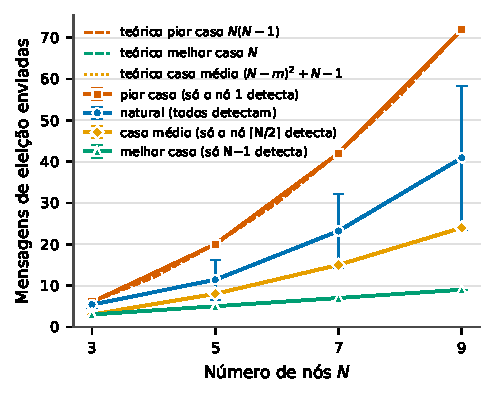
\includegraphics[width=0.48\textwidth]{e1_mensagens_vs_n.pdf}\hfill
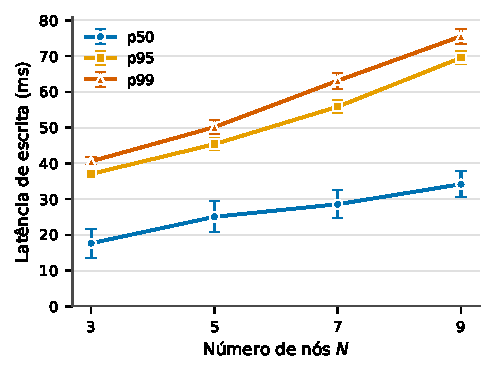
\includegraphics[width=0.48\textwidth]{e2_latencia_vs_n.pdf}
\caption{(a) E1: mensagens da eleição vs.\ $N$ para as quatro variantes e as
curvas teóricas. (b) E2: latência de escrita (p50/p95/p99) vs.\ $N$.}
\label{fig:e1e2}
\end{figure*}

\subsection{E1: tempo e mensagens da eleição}

A Tabela~\ref{tab:e1} mostra que a contagem de mensagens é determinística:
o desvio-padrão foi zero nas 160 réplicas, e os valores coincidem
exatamente com (\ref{eq:bully}). A variante \emph{natural} coincide com o
\emph{pior caso}: com detecção por \emph{timeout} o nó 1 também detecta e a
cascata de \texttt{OK} faz todos os $N-1$ vivos abrirem eleição. Portanto, o
comportamento típico do Valentão aqui já é quadrático (Fig.~\ref{fig:e1e2}a).

\begin{table}[!ht]
\caption{E1: mensagens enviadas na eleição (desvio zero; iguais à teoria). Teoria: $N$, $(N-m)^2+N-1$ com $m=\lceil N/2\rceil$ e $N(N-1)$.}
\label{tab:e1}
\centering
\footnotesize
\setlength{\tabcolsep}{4pt}
\begin{tabular}{@{}rrrrr@{}}
\toprule
$N$ & Melhor & Médio & Pior & Natural \\
\midrule
3 & 3 & 3 & 6 & 6 \\
5 & 5 & 8 & 20 & 20 \\
7 & 7 & 15 & 42 & 42 \\
9 & 9 & 24 & 72 & 72 \\
\bottomrule
\end{tabular}
\end{table}

\begin{table}[!ht]
\caption{E1 (\emph{natural}): tempos em s, média $\pm$ IC95\%.}
\label{tab:e1t}
\centering
\footnotesize
\setlength{\tabcolsep}{3pt}
\begin{tabular}{@{}rllll@{}}
\toprule
$N$ & Detecção & Eleição & Sincr. & \emph{Kill}$\to$pronto \\
\midrule
3 & $0{,}510\pm0{,}024$ & $0{,}303\pm0{,}004$ & $0{,}301\pm0{,}006$ & $1{,}113\pm0{,}025$ \\
5 & $0{,}482\pm0{,}025$ & $0{,}317\pm0{,}013$ & $0{,}304\pm0{,}008$ & $1{,}104\pm0{,}033$ \\
7 & $0{,}470\pm0{,}030$ & $0{,}314\pm0{,}005$ & $0{,}301\pm0{,}007$ & $1{,}085\pm0{,}034$ \\
9 & $0{,}476\pm0{,}020$ & $0{,}311\pm0{,}008$ & $0{,}311\pm0{,}010$ & $1{,}098\pm0{,}024$ \\
\bottomrule
\end{tabular}
\end{table}

Nenhuma fase do tempo cresce com $N$. A detecção ($\approx0{,}47$--$0{,}51$~s)
é $\tau_{fd}$ menos a fase do último \emph{heartbeat}. Eleição e sincronização
duram $\approx\tau_{rpc}=0{,}3$~s, pois as mensagens de uma rodada vão em
paralelo e a rodada só termina quando a chamada ao nó morto estoura o
\emph{timeout}; no Windows, conectar a uma porta fechada leva ${\sim}2$~s (medido),
então só o \emph{timeout} encerra a chamada. O custo $O(N^2)$ aparece em
mensagens, não em latência, em localhost.

\subsection{E2: latência e vazão da escrita}

\begin{table}[!ht]
\caption{E2: latência (ms), vazão (ops/s) e mensagens por escrita; média $\pm$ IC95\% das 10 réplicas.}
\label{tab:e2}
\centering
\scriptsize
\setlength{\tabcolsep}{2pt}
\begin{tabular}{@{}lrllllr@{}}
\toprule
Config. & Vazão & p50 & p95 & p99 & Msg./esc. \\
\midrule
$N{=}3$, 0 ms & $50{,}2\pm3{,}1$ & $17{,}7\pm4{,}1$ & $37{,}0\pm0{,}5$ & $40{,}6\pm1{,}1$ & 4 \\
$N{=}5$, 0 ms & $37{,}8\pm3{,}1$ & $25{,}0\pm4{,}3$ & $45{,}4\pm1{,}7$ & $50{,}1\pm1{,}9$ & 8 \\
$N{=}7$, 0 ms & $32{,}3\pm2{,}3$ & $28{,}6\pm4{,}0$ & $55{,}9\pm1{,}8$ & $63{,}1\pm2{,}2$ & 12 \\
$N{=}9$, 0 ms & $26{,}2\pm1{,}6$ & $34{,}2\pm3{,}6$ & $69{,}5\pm1{,}8$ & $75{,}6\pm2{,}0$ & 16 \\
$N{=}5$, 5 ms & $27{,}7\pm0{,}9$ & $35{,}0\pm2{,}1$ & $55{,}7\pm1{,}9$ & $61{,}8\pm1{,}3$ & 8 \\
$N{=}5$, 20 ms & $14{,}1\pm0{,}3$ & $71{,}8\pm2{,}1$ & $88{,}8\pm1{,}8$ & $93{,}2\pm2{,}6$ & 8 \\
\bottomrule
\end{tabular}
\end{table}

Mensagens por escrita foram \emph{exatamente} $2(N-1)$, com desvio zero nas 60
réplicas. A latência cresce com $N$ (p50 de 17,7 para 34,2~ms de $N=3$ a 9),
porque o primário abre $N-1$ conexões e trata $N-1$ \texttt{ACK} no mesmo laço
de eventos, e com o atraso injetado: a cada escrita ele soma $\approx2\times$ o
atraso nominal (ida do \texttt{REPLICAR} e volta do \texttt{ACK}, com os
backups em paralelo). A vazão cai na mesma proporção, pois há um cliente
síncrono e o primário serializa as escritas. A latência absoluta é alta
($\ge17$~ms) porque cada mensagem abre uma conexão TCP, o que no Windows é caro;
vale a tendência, e os valores absolutos não se transferem a Linux ou a
contêineres.

\subsection{E3: \emph{failover} e falsas suspeitas}

\begin{figure*}[!t]
\centering
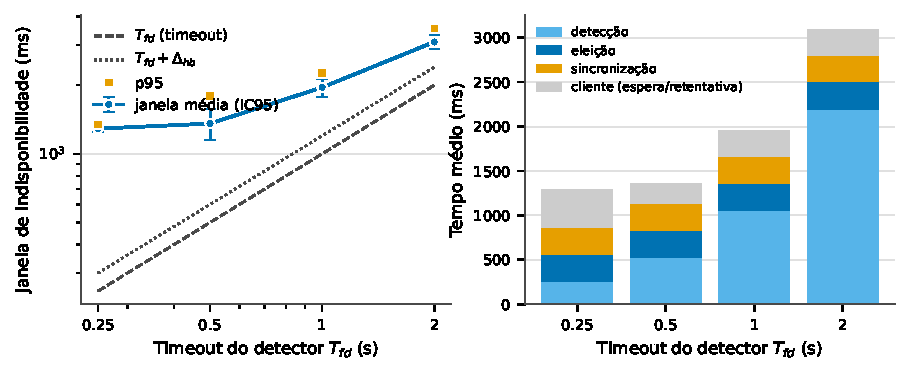
\includegraphics[width=0.49\textwidth]{e3a_janela_vs_timeout.pdf}\hfill
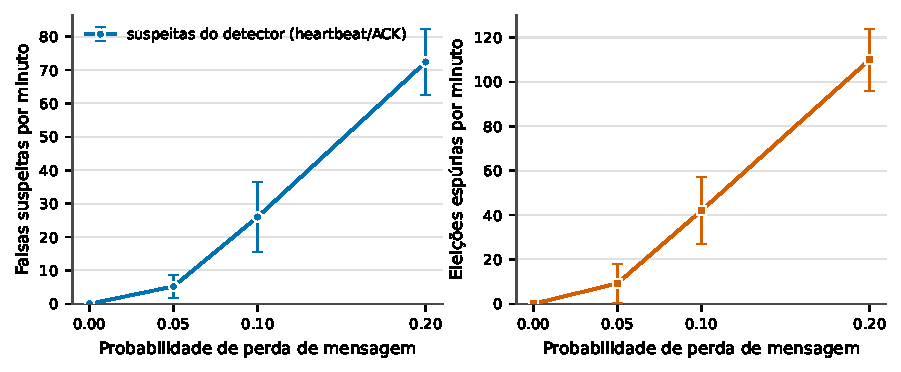
\includegraphics[width=0.49\textwidth]{e3b_falsas_suspeitas_vs_perda.pdf}
\caption{(a) E3a: janela de indisponibilidade e decomposição vs.\
$\tau_{fd}$. (b) E3b: suspeitas falsas vs.\ perda de mensagens.}
\label{fig:e3}
\end{figure*}

\begin{table}[!ht]
\caption{E3a: indisponibilidade após o crash do primário ($N=5$), em s.}
\label{tab:e3a}
\centering
\footnotesize
\setlength{\tabcolsep}{3pt}
\begin{tabular}{@{}rlllll@{}}
\toprule
$\tau_{fd}$ & Detecção & \emph{Kill}$\to$pronto & Janela (média $\pm$ IC) & p50 & p95 \\
\midrule
0,25 & 0,255 & 0,859 & $1{,}29\pm0{,}04$ & 1,30 & 1,34 \\
0,5 & 0,522 & 1,137 & $1{,}36\pm0{,}21$ & 1,18 & 1,79 \\
1,0 & 1,052 & 1,664 & $1{,}96\pm0{,}18$ & 1,78 & 2,26 \\
2,0 & 2,189 & 2,803 & $3{,}10\pm0{,}22$ & 2,92 & 3,54 \\
\bottomrule
\end{tabular}
\end{table}

A janela vista pelo cliente é $\approx\tau_{fd}$ mais eleição e sincronização
(${\approx}2\tau_{rpc}$) mais a retentativa do cliente: a detecção segue
$\tau_{fd}$, e há um piso fixo de ${\sim}0{,}6$~s de eleição e sincronização
(esperam o \emph{timeout} do nó morto; $\tau_{rpc}$ não foi variado). A janela
excede o \emph{kill}$\to$pronto em 0,2 a 0,45~s, pois a tentativa ao primário
morto só falha após o \emph{timeout} de 0,5~s do cliente. Esse timeout é o
piso que torna as janelas em $\tau_{fd}=0{,}25$ e $0{,}5$~s quase iguais, e a
retentativa gera a bimodalidade (p50 abaixo da média em 0,5 e 1~s). Nenhuma
escrita falhou (o cliente repete) e nenhuma confirmada se perdeu.

\begin{table}[!ht]
\caption{E3b: sem crash, $N=5$, janela de 15~s. Suspeitas do detector e eleições espúrias por minuto (média $\pm$ IC95\%).}
\label{tab:e3b}
\centering
\footnotesize
\setlength{\tabcolsep}{3pt}
\begin{tabular}{@{}rllrr@{}}
\toprule
Perda & Susp./min & Eleições esp./min & Troca de líder & Escritas ok \\
\midrule
0 & 0 & 0 & 0 & 188 \\
0,05 & $5{,}2\pm3{,}3$ & $9{,}2\pm8{,}6$ & 0 & 75 \\
0,10 & $26{,}0\pm10{,}6$ & $42{,}0\pm15{,}0$ & 0,4 & 47 \\
0,20 & $72{,}4\pm10{,}0$ & $110\pm14$ & 0,8 & 15 \\
\bottomrule
\end{tabular}
\end{table}

Sem perda, não houve falsa suspeita. A taxa cresce \emph{mais que
linearmente} com a perda (Tabela~\ref{tab:e3b}, Fig.~\ref{fig:e3}b): um seguidor só suspeita após
${\sim}5$ \emph{heartbeats} seguidos sem chegar, e a perda também derruba os
\texttt{ACK} e as mensagens de eleição, o que realimenta o processo. Quase
não há troca de líder: o líder, ao receber \texttt{ELEICAO}, responde com
\emph{heartbeat} em vez de reeleger, e as épocas impedem dois primários. O
efeito visível é na vazão: cada \texttt{REPLICAR} ou \texttt{ACK} perdido
custa um $\tau_{rpc}$ (0,3~s) e a remoção do backup da visão (reentrada por
\texttt{ENTRAR}), e o commit exige quórum; assim, as escritas confirmadas
caem de 188 para 15 em 15~s com 20\% de perda, sem perder nenhuma confirmada.

\subsection{E4: partição do primário}

\begin{table}[!ht]
\caption{E4: primário (nó 5) isolado por ${\approx}4$~s ($N=5$, 10 réplicas).}
\label{tab:e4}
\centering
\footnotesize
\setlength{\tabcolsep}{3pt}
\begin{tabular}{@{}lr@{}}
\toprule
Métrica & Média $\pm$ IC95\% \\
\midrule
Tentativas de escrita no primário isolado & $55{,}7\pm1{,}4$ \\
Confirmadas pelo primário isolado (\texttt{sem\_quorum}) & $0\pm0$ \\
Maioria: nó 4 pronto após o isolamento (s) & $1{,}131\pm0{,}014$ \\
Confirmadas no lado majoritário (de 20) & $20\pm0$ \\
Nó 5 renuncia após curar (s) & $0{,}261\pm0{,}064$ \\
Nó 5 retoma a liderança (s) & $0{,}487\pm0{,}090$ \\
Convergência total após curar (s) & $0{,}627\pm0{,}098$ \\
Escritas órfãs no estado final & 0 \\
\bottomrule
\end{tabular}
\end{table}

O primário isolado não confirmou nenhuma das ${\sim}56$ tentativas, todas
respondidas com \texttt{sem\_quorum}; a maioria elegeu o nó 4, que ficou
pronto em ${\sim}1{,}13$~s e confirmou todas as 20 escritas. Ao curar, o nó 5
renunciou pela época maior, retomou a liderança (maior id) e tudo convergiu,
sem escritas órfãs. É o \emph{split-brain} da Seção~IV-A resolvido pelo
quórum, na prática.

\textbf{Correção em todos os experimentos.} Nas 310 réplicas de falha, o
verificador reportou 0 violações (I1--I6) e a checagem do cliente, 0 escritas
confirmadas perdidas.

\FloatBarrier

\section{Limitações}

\textbf{Domínios de falha.} Processos ou contêineres numa só máquina não são
independentes (Seção~II): não há falha correlacionada, latência real de rede
nem perda de disco, e os tempos refletem um único escalonador; os valores
absolutos não se transferem a outro hardware. \textbf{Docker.} O \texttt{compose.yaml} não foi executado por nós (Seção~II).
\textbf{Disponibilidade.} O quórum de maioria sacrifica disponibilidade:
sem a maioria dos nós vivos, não há escritas nem leituras.
\textbf{Perda possível.} Uma escrita confirmada se perde se todos os nós que
a têm morrem ou perdem o disco e os sobreviventes formam quórum; \texttt{kill}
preserva o disco, e \texttt{--fsync} cobre queda da máquina.
\textbf{Leituras.} O \texttt{GET} é no primário, com \emph{lease} de
$\tau_{fd}$; entre a perda de liderança e esse limite, uma leitura obsoleta é
possível, e depende da sincronia parcial. \textbf{Desempenho.} Uma conexão TCP por mensagem e escritas
serializadas no primário privilegiam a simplicidade, não a vazão; o conjunto
de nós é fixo (sem reconfiguração); não se toleram falhas bizantinas.

\section{Conclusão}

Integramos Valentão, primário-backup síncrono e detector por
\emph{heartbeat} em um armazenamento replicado cuja segurança repousa em três
peças: quórum de maioria no commit, épocas e líder reconhecido persistidos e
fase de sincronização pós-eleição. O Valentão pode produzir dois líderes sob
partição, e o heartbeat pode suspeitar de nós vivos; ambos custam apenas
vivacidade, pois só o lado majoritário conclui a sincronização e os demais
são recusados por época. As propriedades são checadas por testes de
integração e pelo verificador de logs, e a campanha as confirmou: em 310
réplicas de falha, houve 0 violações e 0 escritas confirmadas perdidas. O
Valentão custou $N$ mensagens no melhor caso e $N(N-1)$ no pior (também o
caso natural), sem que o tempo de eleição crescesse com $N$; a escrita custou
$2(N-1)$ mensagens; a janela de indisponibilidade foi de $1{,}29$ a $3{,}10$~s
para $\tau_{fd}$ de 0,25 a 2~s; com 20\% de perda, as escritas confirmadas
caíram de 188 para 15 em 15~s, sem perda de dados; e o primário isolado não
confirmou nada.

\section*{Divisão de trabalho}
\noindent\textit{Caique Pinheiro Andrade:} implementação dos algoritmos e da
infraestrutura de comunicação, e execução da campanha experimental.
\textit{Luiz Henrique Marques Gonçalves:} modelo do sistema e argumentos de
correção, análise dos resultados e redação do relatório.

\begin{thebibliography}{9}
\bibitem{vansteen2023} M.~van Steen and A.~S. Tanenbaum, \emph{Distributed
Systems}, 4th~ed. distributed-systems.net, 2023.
\bibitem{garcia1982} H.~Garcia-Molina, ``Elections in a distributed
computing system,'' \emph{IEEE Trans.\ Computers}, vol.~C-31, no.~1,
pp.~48--59, 1982.
\bibitem{budhiraja1993} N.~Budhiraja, K.~Marzullo, F.~B. Schneider, and
S.~Toueg, ``The primary-backup approach,'' in \emph{Distributed Systems},
2nd~ed., S.~Mullender, Ed. ACM Press, 1993, pp.~199--216.
\bibitem{chandra1996} T.~D. Chandra and S.~Toueg, ``Unreliable failure
detectors for reliable distributed systems,'' \emph{J.\ ACM}, vol.~43,
no.~2, pp.~225--267, 1996.
\bibitem{ongaro2014} D.~Ongaro and J.~Ousterhout, ``In search of an
understandable consensus algorithm,'' in \emph{Proc.\ USENIX Annual
Technical Conf.\ (ATC)}, 2014, pp.~305--319.
\end{thebibliography}

\end{document}
